\documentclass[SDSUThesis.tex]{subfiles} 
\begin{document}

\newpage
\pagenumbering{arabic}
\setcounter{tocdepth}{2}

% see this for  guidance https://www.cs.purdue.edu/homes/dec/essay.dissertation.html
\section{INTRODUCTION}

    Software is becoming a vital part of companies. In 2011 Marc Andreessen, 
    co-founder of the venture capital firm Andreessen-Horowitz,
    famously claimed, ``Software is Eating The World'' \cite{Andreessen2001}. 
    His argument was for the ever increasing importance of software
    in all organizations big and small regardless of the industry.  With 
    this important declaration, the production of new software is
    going to be critical.  Just as important will be the effective 
    measurement of how this software is produced.  
    
    This work 
    provides a technique for a software development organization to create
    a single number score which indicates the overall performance
    of the organization. The
    score is based upon data collected for 5 result indicators
    of a software development organization: quality, availability,
    satisfaction, schedule, and requirements.  It is not meant
    to be comparative between organizations, but to 
    form a historical baseline for a specific organization.  

\subsection{OVERVIEW}
    
    Software development organizations are no different than 
    any other business or organization.  There are: tasks
    to be completed, goals to achieve (or miss), and measurements
    to be analyzed.  One difficulty with software development
    is the varied number and amount of measurements to be used. 
    It can be difficult to determine the correct activities
    to measure and the appropriate mechanism to report the measure.
    This has led organizations to either collect too little information
    or to collect too much information.  Another problem is the 
    inconsistency of the reported measures.  It is difficult to compare
    historical performance if the same measurements are not consistent
    throughout the recent history of an organization. 
    
    Software development organizations need a framework to define
    what measurements should be tracked and how those measurements
    should be reported.  The MPI framework provides a solid foundation
    for a consistent evaluation.  MPI analyzes the historical performance
    of an SDO
    to create a baseline in order to provide a broad
    view of the overall organization.  It is common for software development
    organizations to measure and focus soley on the source code
    being produced.  However, a software development organization does more
    than just produce source code.  There is documentation to be
    written, testcases to be created, systems to be deployed, and
    decisions to be made.  The framework provides an evaluation
    of the overall software development organization, not just the
    source code.
    
    The framework will produce a single number score for each of 
    the five result indicators as well as a single overall score.  
    It will be able to provide a quick evaluation of the organization.
    The scores will enable performance to be consistently measured
    and compared.

    Other attempts at evaluating a software development organization
    have been presented, but none produce a single number score for
    the entire effort of the software development organization. 
    The following are attempts to evaluate all or parts of 
    software development.



\subsection{CMMI}
    The Capability Maturity Model Integration (CMMI) is one of the most 
    widely acknowledged models for process 
    improvement in software development.  CMMI offers a generic guideline 
    and appraisal program for process 
    improvement.  It was created and is administered by the 
    Software Engineering Institute at
    Carnegie Mellon University. While the CMMI is not specific to software development,
    it is often applied in software development settings.
    CMMI certification is required for many United States Government 
    and Department of Defense contracts. 
    
    CMMI-Dev is a modification of the CMMI specific to the 
    development activities applied to products
    and services \cite{CMMI}.  The practices covered in 
    CMMI-Dev include project management, 
    systems engineering, hardware engineering, process 
    management, software engineering, and 
    other maintenance processes.  Five maturity levels are 
    specified, and they include the 
    existence of a number of process areas.  The 5 maturity 
    levels and the process areas are specified as follows.

    \begin{description}
        \item[CMMI MATURITY LEVEL 1 - INITIAL]
            A maturity level 1 organization consists of an
                adhoc and chaotic processes.  While working
                products are still produced, the results are 
                often over budget and behind schedule.  A level
                1 organization will also have difficulties 
                repeating a process with the same degree of 
                success.  These organizations typically rely 
                on the heroic efforts of certain individuals. 
            
        \item[CMMI MATURITY LEVEL 2 - MANAGED]
            A maturity level 2 organization has a policy for 
            planning and executing processes.  
            The processes are controlled, monitored, 
            reviewed, and enforced.  The practices are even
            maintained in times of stress.  The following 
            process areas should be present at maturity
            level 2.
            \begin{itemize}
                \item Configuration Management (CM)
                \item Measurement and Analysis (MA)
                \item Project Monitoring and Control (PMC)
                \item Project Planning (PP)
                \item Process and Product Quality Assurance (PPQA)
                \item Requirements Management (REQM)
                \item Supplier Agreement Management (SAM)
            \end{itemize}

        \item[CMMI MATURITY LEVEL 3 - DEFINED]
            A maturity level 3 organization has well-understood 
            processes that are described in 
            standards, tools, procedures, and methods.  The 
            organization has standard processes
            that are reviewed and improved over time.  The 
            major differentiators between level 2 
            and level 3 is the existence of standards and process descriptions. 
            A level 2 organization will have
            processes that are inconsistent across projects.  
            A level 3 organization will tailor
            a standard process for each project.  Also, 
            level 3 processes are described with 
            much more rigor.  In addition to the process areas found in level 2, 
            the following process areas should be present at maturity level 3.
            \begin{itemize}
                \item Decision Analysis and Resolution (DAR)
                \item Integrated Project Management (IPM)
                \item Organizational Process Definition (OPD)
                \item Organizational Process Focus (OPF)
                \item Organizational Training (OT)
                \item Product Integration (PI)
                \item Requirements Development (RD)
                \item Risk Management (RSKM)
                \item Technical Solution (TS)
                \item Validation (VAL)
                \item Verification (VER)
            \end{itemize}
            
        \item[CMMI MATURITY LEVEL 4 - QUALITATIVELY MANAGED]
            A maturity level 4 organization has quantitative 
            measures for quality and process performance. 
            The measures are based upon customer needs, 
            end users, and process implementers.  
            The quality
            and process performance are understood mathematically and managed 
            throughout the life of a project.
            Level 4 is characterized by the predictability of the process performance. 
            In addition to
            the process areas found in level 2 and 3, the following additional 
            process areas should be present
            at maturity level 4.
            \begin{itemize}
                \item Organizational Process Performance (OPP)
                \item Quantitative Project Management (QPM)
            \end{itemize}
            
        \item[CMMI MATURITY LEVEL 5 - OPTIMIZING]
            The final and pinnacle level of CMMI maturity is level 5.  
            A maturity level 5 organization
            continually improves processes based upon quantitative measures.  
            The major distinction from 
            level 4 is the constant focus on improving and managing 
            organizational performance.  A maturity level
            5 organization has well-documented standard processes that are 
            tracked and enforced as well as
            a focus on continual improvement of the processes based upon 
            quantitative measures.  In addition to the process areas of the 
            previous maturity levels, maturity
            level 5 should contain the following process areas.
            \begin{itemize}
                \item Causal Analysis and Resolution (CAR)
                \item Organizational Performance Management (OPM)
            \end{itemize}
    \end{description}

    \begin{figure}[ht]
        \centering
        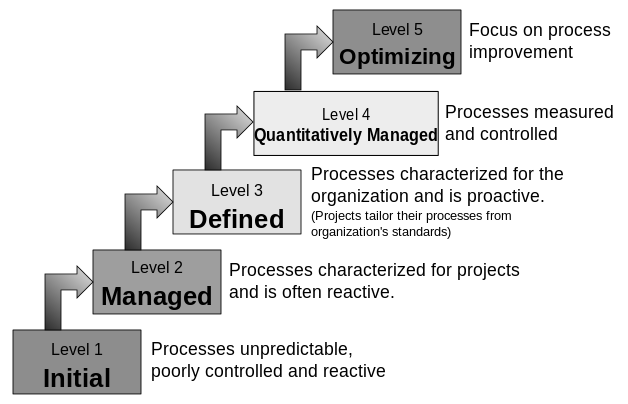
\includegraphics[scale=.7]{images/cmmi.png}
        \caption[CHARACTERISTICS OF CMMI]{Characteristics of CMMI, 
            image adapted from  \cite{Godfrey} }
        \label{fig:cmmi}
    \end{figure}

    A visual description of the CMMI maturity levels can be seen in Figure \ref{fig:cmmi}.  
    While CMMI-Dev does provide an excellent framework for improving a process.  It
    is wholely focused on process improvement.  It does not provide guidelines
    for evaluating the final product.  
    Also, it does not provide a specify mechanism for evaluating
    or scoring the progression through the maturity levels.  
    An indicator is still needed to quantify the overall 
    performance of an organization, not
    just the compliance to standard processes.  


\subsection{PREVIOUS SOFTWARE EVALUATION WORK}

    An example of scoring software development is presented by 
    Jones \cite{Jones2012}. The methodology looks
    for the presence of various techniques used in software engineering.  
    The methodology provides a score based upon the 
    productivity and quality increase of the technique being evaluated.  
    Points are positive or negative based upon the 
    presense of various techniques. A couple example techniques are: 
    automated source code analysis and continuous integration.  The end 
    result is a score in range $[-10,10]$. 
    While the result is a single number score, it does not account for the 
    entirety of the software development lifecycle.

    Constructive Cost Model (COCOMO) is a software cost estimation model created
    by Boehm \cite{Boehm1981}.  It combines future project characteristics
    with historical project data to create a regression model to estimate the 
    cost of a software project.  The original version developed in 1981 was
    focused on mainframe and batch processing.  An unpdated version, named
    COCOMO II, was created by Boehm in 1995 to be more flexible for newer 
    development practices such as desktop development, off the shelf components,
    and code reuse.  COCOMO provides a nice algorithm for making decisions
    regarding building or buying software products.  It does not provide 
    an algorithms to review past performance of estimates and modify the
    algorithm accordingly.  COCOMO II can be a useful tool for 
    estimating the time and costs within an SDO,
    but it only provides an estimate and not an evaluation of the actual
    performance. 
    
    Sextant is a visualization tool for Java source code \cite{Winter2013}.  
    Sextant provides a graphical representation of the information related 
    to a software system.  The tool provides the capability to provide 
    custom rules which are specific to the domain or application.  However,
    Sextant only provides metrics and analysis of the software code.  
    It provides no information regarding the rest of the 
    software development lifecycle.  Also, the primary output of Sextant 
    is visual graphs.  While these graphs do provide
    useful information, they do not provide a single number 
    to determine the performance of the software.

    Another promising research area is \textit{process mining}.
    As stated by Wil van der Aalst \cite{vanderAalst2011}, 
    ``The idea of process mining is to discover, monitor
    and improve real
    processes (i.e., not assumed processes) by extracting knowledge from event logs
    readily available in today's systems.''  Creating software involves
    a vast amount of processes.  Numerous logs of raw data are collected.  
    One application of process mining in the area of software development
    was an algorithm and information for measuring a software engineering process from
    the Software Configuration Management (SCM) \cite{Rubin2007}.
    The technique creates process models 
    to understand the process of developing software and code. 
    It is less focused on the output and results,
    but it is more focused on adherence to a specified process.
    
    Process mining has also been applied to decision making regarding software 
    upgrades \cite{Genuchten2014}.  Historic and current logs can be 
    processed and evaluated.
    Then small pilot groups can be offered the upgrade, and the new logs will 
    be processed and evaluated. Thus, process mining can be beneficial for new 
    software implementation.  More research needs to be done applying
    process mining to the other process involved with software development,
    such as other documentation, testing, and implementation. 
    
    Although process mining can be useful for analyzing software
    development data, it has not yet been applied to the entirety 
    of a software development organization. It also does not
    focus on the results of the organization.  It focuses
    on process conformance, which can be very important, so it
    is limited in the ability to evaluate the entire organization. 

    Much work has been done to determine metrics for source code, in fact 
    entire books have been written on the topic of software 
    metrics \cite{Jones1996, Putnam2013}. Yet, 
    organizations still struggle to measure the production of software.
    Little work exists
    for scoring the entire software development organization. 

\subsubsection{SEMAT}

    Software Engineering Method and Theory (SEMAT) is claiming to 
    be the ``new software engineering'' 
    \cite{Jacobson2014}.  The authors rightfully claim that 
    software engineering lacks
    an underlying theoretical foundation found in other 
    engineering disciplines.  This lack of theory
    has led software engineering to not be engineering, but 
    rather a craft.  The goal of 
    SEMAT is to merge the craftsmanship and engineering to 
    provide a foundation for software
    engineering.  The primary initiative of SEMAT 
    has been the creation of a kernel for 
    software engineering.  The kernel is the minimal set 
    of things common to all software development
    endeavours. The three parts to the kernel are:
    \begin{description}
        \item[Measurement] - There must exist a means to 
            determine the health and progress of an endeavour
        \item[Categorization]-  The activities must progress 
            through categories during an endeavour
        \item[Competencies] - Specific competencies will 
            be required for completing activities
    \end{description}
    
    The kernel defines alphas, which are seven dimensions with
    specific states for measuring progress. 
    The seven dimensions are: 
    \begin{enumerate}
        \item Opportunity
        \item Stakeholders
        \item Requirements
        \item Software Systems
        \item Work
        \item Team
        \item Way of Working
    \end{enumerate}
    
    Although SEMAT is very promising, the development is not yet complete.  Adoption is
    limited so the technique has not been validated on many
    actual software engineering endeavours.  Although SEMAT does include a part for
    measurement of progress, it does not specify how the measurement is to be 
    performed.

\subsubsection{SOFTWARE QUALITY}

    Software quality is one of the most well studied aspects
    of software development.  Most of the work focuses on
    either the problems with the software or the source code.
    Quality and the number of problems with the software
    are inversely related, more problems means lower quality. 
    Quality is easy to measure, but 
    that measurement is usually very software specific.  It is easy
    to find that some software has $X$ number of problems, but
    it is nearly impossible to determine whether the quality
    of that software is better or worse than some other software
    with $X$ defects.  One piece of software can be 
    larger\footnote{Saying a piece of software is larger can be a 
    rather arbitrary statement.  Does that mean the software requires 
    more computing time, has more lines of code, more documentation, 
    more hours spent on development, or some other arbitrary measure.}
    or more complex.  Thus, finding a value for quality is easier 
    than interpreting that value.  Not matter the interpretation,
    the goal is to release the number of problems with the software.
    Top 10 lists have been created for techniques to remove problems
    from software \cite{Boehm2001}.  
    A number of different techniques or best practices
    for preventing defects have 
    been proposed \cite{Faizan2012}.  These are all strategies to identify
    or remove the problems before the software is completed and released
    to users.  
    
    Another aspect of software quality is the complexity of the 
    source code.  More complex code results in more maintenance efforts and
    more chances for problems. A couple of numerical measures for the 
    complexity of source code have been created.  The most common examples
    are McCabe \cite{McCabe1976} and Halstead \cite{Halstead1977}.
    However, the measures on source code only explain part of the 
    software development lifecycle.  
    
    Another measurement of quality can be the cost per defect, also 
    known as the cost to fix a problem.  As seen in \cite{Jones2013},
    this measurement has problems because the lowest cost per
    defect will occur on software with the most problems.  Therefore,
    the lowest cost per defect is actually the lowest quality as well.
    Due to this difficulty and others, a number of other models
    have been created for evaluating the quality of software 
    \cite{Miguel2014}.  While all of the models have merit
    in certain situations, the measures of quality must be combined
    with other measures in order to provide an overall evaluation
    of a software development organization.
    

\subsubsection{SOFTWARE ANALYTICS}

    One area of research that is focusing on the evaluation 
    of software development organizations
    is \textit{software analytics}. 
    Software analytics is less focused on evaluation
    and more so on all sorts of analysis of software data.
    The earliest variants
    of software analytics were disguised as
    applications of data mining techniques to software 
    engineering data in the 
    late 1990s \cite{Ruhe1997,Ebert1999,Goel1997}.   
    Later the field began to emerge more heavily, but still
    remained primarily methods of data mining applied to 
    software engineering \cite{Kaner2004,Xie2009,Taylor2010,Halkidi2011}. 
    Finally, The term software intelligence was proposed for the field of study
    \cite{Hassan2010}, but eventually
    the term software analytics became the dominant term for referring to the 
    field of study \cite{Buse2010, Zhang2011}.
    
    The goal of software analytics is to extract insights
    from software artifacts to aide practitioners in making 
    better decisions regarding software
    development \cite{Zhang2013}.  The three main focus areas of 
    software analytics are:
    \begin{description}
        \item[User Experience] - How can the software enable the 
            user to more easily or quickly 
            accomplish the task at hand?
        \item[Quality] - How can the number of problems with 
            the software be decreased?
        \item[Development Productivity] - How can the processes
            or tools be modified to increase 
            the rate at which software is produced? 
    \end{description}
    The work presented later in this paper will address all three
    focus areas.  

    Martin Shepperd in \cite{Hassan2013} identified 3 important questions that software
    analytics must address:
    \begin{enumerate}
        \item ``How much better is my model performing than 
            a naive strategy, such as guessing [\ldots]?''
        \item ``How practically significant are the results?''
        \item ``How sensitive are the results to small changes in 
            one or more of the inputs?''
    \end{enumerate}
    These are 3 important questions that should be addressed 
    when presenting any results in software analytics.  The research
    needs to demonstrate clear advantages for practitioners.

    One of the software analytic techniques focuses specifically 
    on the source code; analyzing the 
    complexity, size, and coupling \cite{Tosi2012}. 
    Letier and Fitzgerald discuss how to choose the 
    correct tools and techniques to analyze
    software data \cite{Letier2013}.  A goal model is 
    produced that matches the data analysis methods
    with the goals of the software stakeholders. The method does not focus
    specifically on analysis of the development of software.
    
    \textit{Software Development Analytics} is a subfield of 
    software analytics \cite{Menzies2012}.  It focuses
    specifically on the 
    analytics of the development of software, however not
    the overall performance of the software.  Hassan points out
    in \cite{Hassan2013} that software analytics needs to go beyond
    just the developers.  Everyone and everything involved in the 
    development of software produces some data and that data can be meaningful.
    The insights from non-developer data has the potential to yield important
    results as well. 
    Software development produces many valuable pieces of datum that can be analyzed
    \cite{Marcus2010}. Just a few of the pieces of datum are:
    email communication, bugs, fixes, source code, version control system histories,
    process information, and test data.  Examples of this type of data
    can be found in the PROMISE Data Repository \cite{promise12}.
    
    All of these techniques are of no use if the correct data
    is not available.  Therefore, it is important to 
    identify the information that is needed to properly 
    perform software development analytics.
    Unfortunately, there are vast amounts of information that 
    need to be collected to meet the analytic needs of 
    developers and managers \cite{Buse2012}.  When the
    data and tools exists, the analytics should help an
    organization with the following tasks.
    \begin{itemize}
        \item Evaluate a project
        \item Determine what is and is not working
        \item Manage Risk
        \item Anticipate changes
        \item Evaluate prior decisions
    \end{itemize}
    
    In order to store the data, appropriate tools are needed.  Microsoft
    is working on developing some tools for the analysis of the development
    of software \cite{Czerwonka2013,Zhang2013}.  Microsoft has developed
    StackMine, a postmortem tool for performance debugging, and CODEMINE,
    a tool for collecting and analyzing software development process data.
    Both tools provide analytical insight for various aspects of the 
    software development process, however neither tool covers all aspects
    of software development.
    These tools are currently early in development and the adoption of the
    tools by practitioners is still unknown. One of the reasons for the slow
    adoption of new tools is the inherent difficulty of producing
    new tools for the software development process \cite{Spraragen2005}. A 
    tool that works fantastic for one team might not automatically apply to 
    another team.  The people creating the tools need to be acutely aware
    of the needs of the technical practitioners that will be using the
    tools.  

    After the proper tools are in place to collect the necessary
    data on software development and software analytics are being
    properly implemented, an obvious next step is the
    application of gamification to software development. Gamification
    is ``the process of making activities more game-like'' \cite{Werbach2014}.
    some of the benefits of gamification are higher productivity, competition,
    and greater enjoyment.  
    Prior attempts
    at gamification of software development focus only on 
    the computer programming phase \cite{Snipes2013}. Others
    focus on defining a framework for gamification within
    the software development process \cite{Jain2013}. There are 
    even some indications that gamification might help increase
    software quality \cite{Dubois2013}. 
    While this work will not focus on gamification, it is important to note
    that an implementation of an evaluation technique for software
    development could be implemented simultaneously with a gamification
    strategy. Both will require new collections of data and new reporting.

    So it has been shown, there exist many attempts to 
    evaluate portions of the a software development 
    organization.  None of the the attempts provide
    a single number score for the entirety of the 
    organization.  Most of the techniques focus on
    specific portions of the software development 
    lifecycle, namely the development portion. Plus,
    there are many tools that need to be created for
    software analytics to provide all the value
    that it promises.

\subsection{ORGANIZATION OF THE WORK}

The remainder of this dissertation is divided into 5 chapters.  The next chapter provides
an overview of software, software development lifecycles, software engineering, and software
development organizations.  Chapter 3 introduces what is meant by the term data-driven
software engineering. Chapter 4 then provides an explanation of the Master Performance 
Indicator (MPI).  It will present the essential elements for calculating the MPI, as well
as the formulas, frameworks, and data necessary to produce the MPI. Chapter 5 provides
a technological framework for generating and storing the current and historical MPI values.
Chapter 6 demostrates how MPI can be implemented in a software development portion of 
a large financial institution.  Chapter 7 concludes the dissertation with a summary
of the results and some possible future directions for further enhancements. 

\end{document}